%! Author = adnansiddiquei
%! Date = 20/12/2023

\subsection{Q4 - Baseline Dataset}\label{subsec:q4}
\subsubsection{Question 4a}\label{subsubsec:q4a}
    Classification decision trees utilise recursive binary splitting to split the feature-space into high dimensional
    rectangles in order to predict the outcome class given a feature set.
    In each iteration, an existing rectangle is split into two new rectangles, by splitting on a feature and a threshold
    value for that feature.
    The end tree will have some number of internal nodes $N_{n}$, representing splits in the feature space, and $N_{n} + 1$
    terminal nodes which represent the final classification, which would be the modal class in that rectangle.
    The quality of the split can be measured by a criterion such as the Gini index, and at each split, the feature to
    split on and the threshold would be chosen by whichever split decreases the Gini index the most.
    The Gini index is defined as \cite{ISL}:
    \begin{equation}
        G = \sum_{k=1}^{K} \hat{p}_{mk}(1 - \hat{p}_{mk})
        \label{eq:gini-index}
    \end{equation}
    where $\hat{p}_{mk}$ is the proportion of training samples in the $m$th region that are from the $k$th class.
    A region $m$ that contains mainly a single class will have a small Gini index for that region.

    Decision trees suffer from high variance as the trained model is highly dependent on the training data.
    Bagging and random forests are ensemble methods that reduce the variance of decision trees.
    With bagging, multiple decision trees are trained on different bootstrapped samples of the training data, and the
    classification is then decided by a majority vote of the trees.
    Random forests reduce the variance further by forcing an internal node to split on a random subset of the features,
    resulting in less correlated trees, and therefore a larger decrease in variance.

    Two hyperparameters of random forests \inlinecode{max_depth} and \inlinecode{max_features}, the former is the
    maximum number of internal nodes per tree, and the latter is the number of features to consider when splitting.
    Heuristically, \inlinecode{max_depth} is typically set to $\sqrt{N}$ where $N$ is the number of features.

\subsubsection{Question 4b, 4c, 4d and 4e}\label{subsubsec:q4bcde}
    The dataset was pre-processed using the same outlier removal technique as in Section \ref{subsubsec:q3de}, and then
    standardised.
    No duplicates or missing values were found.
    The dataset contained imbalanced classes, as such, stratified sampling was used for train-test splitting.

    \begin{figure}[htb]
    \centering
    \begin{subfigure}{0.5\textwidth}
        \centering
        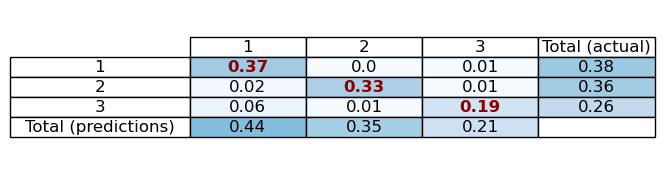
\includegraphics[width=0.9\textwidth]{./figures/q4c_confusion_matrix}
        \caption{Mean confusion matrix.}
        \label{fig:q4c_confusion_matrix}
    \end{subfigure}%
    \begin{subfigure}{0.5\textwidth}
        \centering
        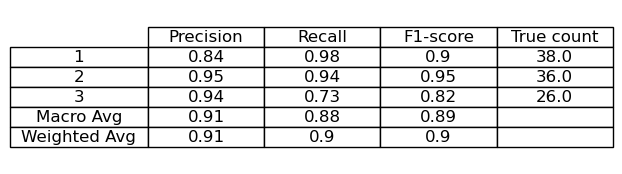
\includegraphics[width=0.9\textwidth]{./figures/q4c_classification_report}
        \caption{Mean classification report.}
        \label{fig:q4c_classification_report}
    \end{subfigure}
    \caption{Confusion matrix and classification report averaged over 5-folds of cross validation for the random forest
        classifier on \inlinecode{ADS_baselineDataset.csv}. The leading diagonal of the confusion matrix indicates a
        mean 10.0\% test set classification error.
        The confusion matrix cells are shown as percentages of the total number of samples in the test set.
        The train test split was 0.8/0.2, giving a test set size of 100.}
    \label{fig:q4c}
    \end{figure}

    The dataset was then classified using \inlinecode{RandomForestClassifier} and Fig.\eqref{fig:q4c} shows a summary
    of the model performance, averaged over 5-folds of cross validation.
    This gave a test set classification error of 11\%.

    \begin{figure}[htb]
    \centering
    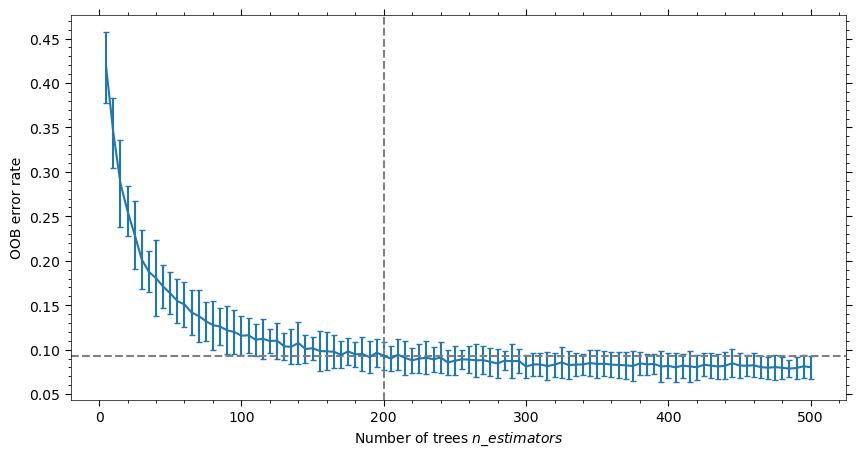
\includegraphics[width=0.9\textwidth]{./figures/q4d}
    \caption{The out of bag error rate for a \inlinecode{RandomForestClassifier} on the pre-processed dataset
        \inlinecode{ADS_baselineDataset.csv}. The OOB error rate was computed 20 times at each value of
        \inlinecode{n_estimators} to give error bars.}
        \label{fig:q4d}
    \end{figure}

    \begin{figure}[htb]
    \centering
    \begin{subfigure}{0.5\textwidth}
        \centering
        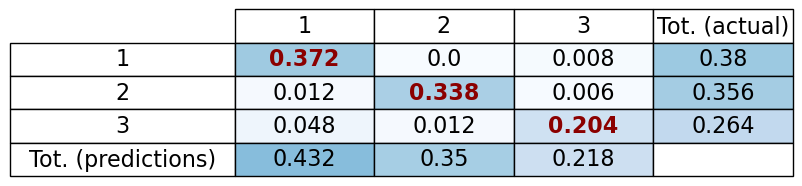
\includegraphics[width=0.9\textwidth]{./figures/q4d_confusion_matrix_200_trees}
        \caption{Mean confusion matrix.}
        \label{fig:q4d_confusion_matrix_200_trees}
    \end{subfigure}%
    \begin{subfigure}{0.5\textwidth}
        \centering
        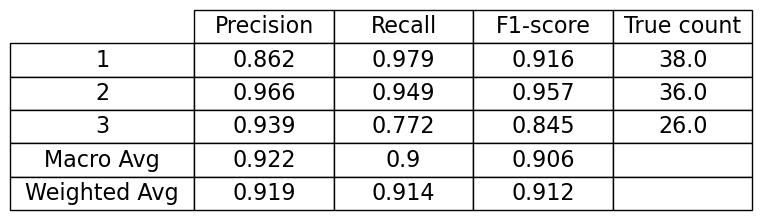
\includegraphics[width=0.9\textwidth]{./figures/q4d_classification_report_200_trees}
        \caption{Mean classification report.}
        \label{fig:q4d_classification_report_200_trees}
    \end{subfigure}
    \caption{The results shown in Fig. \eqref{fig:q4c} but with 200 trees. The mean test set classification error was
        8.6\%.}
    \label{fig:q4d_200_trees}
    \end{figure}

    The \inlinecode{RandomForestClassifier} was then optimised using the out-of-bag (OOB) error rate, the results of this
    is shown in Fig. \eqref{fig:q4d} where it was found that after 200 trees, the OOB error rate did not decrease by
    any significant amount.
    Fig. \eqref{fig:q4d_200_trees} shows the summary of the model performance with 200 trees.
    The test set classification error marginally improved to 9\% and the average precision, recall and F1-scores also
    marginally improved.
    These results are in line with Fig. \eqref{fig:q4d} which shoes a noticeable but not significant decrease in the
    OOB error rate from 100 to 200 trees.

    \begin{figure}[htb]
    \centering
    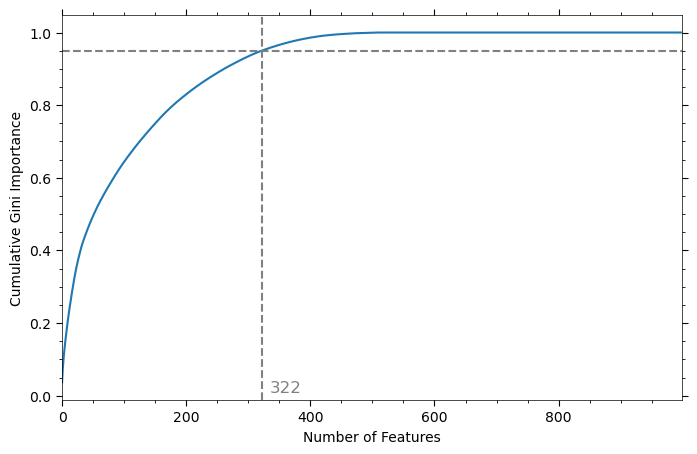
\includegraphics[width=0.9\textwidth]{./figures/q4e_gini_importance}
    \caption{The ordered (highest first), cumulative Gini importance of the features in
        \inlinecode{ADS_baselineDataset.csv}. The horizontal grey line is the 95\% threshold, which contains the top
        322 features.}
        \label{fig:q4e_gini_importance}
    \end{figure}

    \begin{figure}[htb]
    \centering
    \begin{subfigure}{0.5\textwidth}
        \centering
        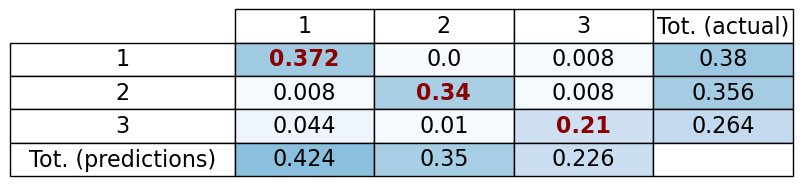
\includegraphics[width=0.9\textwidth]{./figures/q4e_confusion_matrix}
        \caption{Mean confusion matrix.}
        \label{fig:q4e_confusion_matrix}
    \end{subfigure}%
    \begin{subfigure}{0.5\textwidth}
        \centering
        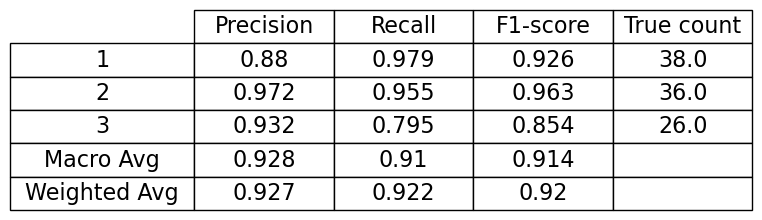
\includegraphics[width=0.9\textwidth]{./figures/q4e_classification_report}
        \caption{Mean classification report.}
        \label{fig:q4e_classification_report}
    \end{subfigure}
    \caption{The results shown in Fig. \eqref{fig:q4c} and Fig. \eqref{fig:q4d_200_trees} but with 200 trees and
        utilising only the top 322 features. The mean test set classification error was 7.8\%.}
    \label{fig:q4e}
    \end{figure}

    The feature importance was then computed using the Gini importance given within
    \inlinecode{RandomForestClassifier.feature_importances_} as shown in Fig. \eqref{fig:q4e_gini_importance}.
    The Gini importance of a feature is defined as the total (normalised) decrease in the Gini index as a result of all
    internal splits within trees that split on a given feature, so a feature is more important if it is used in many
    splits, and if these splits consequently result in a large decrease in the Gini index.
    The top 322 features containing 95\% of the cumulative Gini importance were then selected to redo the classification,
    and the results are shown in Fig.\eqref{fig:q4e}.
    Fig.\eqref{fig:q4e}, when compared to Fig.\eqref{fig:q4d_200_trees}, shows that equivalent (or marginally better)
    performance is achievable by only using the subset of most important features.

\subsubsection{Question 4f}\label{subsubsec:qf}
    \begin{figure}[htb]
    \centering
    \begin{subfigure}{0.5\textwidth}
        \centering
        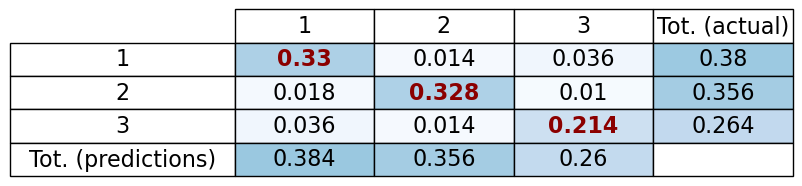
\includegraphics[width=0.9\textwidth]{./figures/q4f_confusion_matrix_all_feats}
        \caption{Mean confusion matrix.}
        \label{fig:q4f_confusion_matrix_all_feats}
    \end{subfigure}%
    \begin{subfigure}{0.5\textwidth}
        \centering
        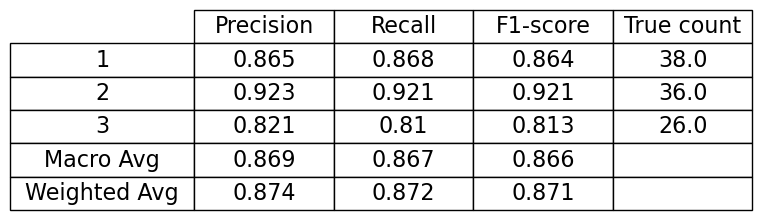
\includegraphics[width=0.9\textwidth]{./figures/q4f_classification_report_all_feats}
        \caption{Mean classification report.}
        \label{fig:q4f_classification_report_all_feats}
    \end{subfigure}
    \caption{Confusion matrix and classification report averaged over 5-folds of cross validation for the
        \inlinecode{LogisticRegression} classifier on \inlinecode{ADS_baselineDataset.csv}.
        The leading diagonal of the confusion matrix indicates a mean 12.8\% test set classification error.
        The confusion matrix cells are shown as percentages of the total number of samples in the test set.
        The train test split was 0.8/0.2, giving a test set size of 100.}
    \label{fig:q4f_all_feats}
    \end{figure}

    \begin{figure}[htb]
    \centering
    \begin{subfigure}{0.5\textwidth}
        \centering
        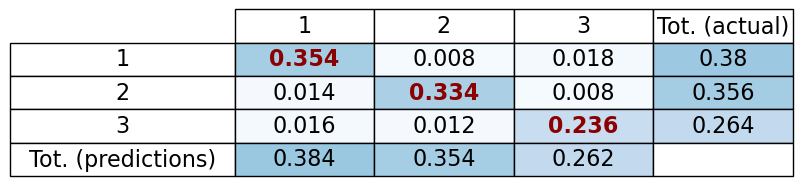
\includegraphics[width=0.9\textwidth]{./figures/q4f_confusion_matrix_reduced_feats}
        \caption{Mean confusion matrix.}
        \label{fig:q4f_confusion_matrix_reduced_feats}
    \end{subfigure}%
    \begin{subfigure}{0.5\textwidth}
        \centering
        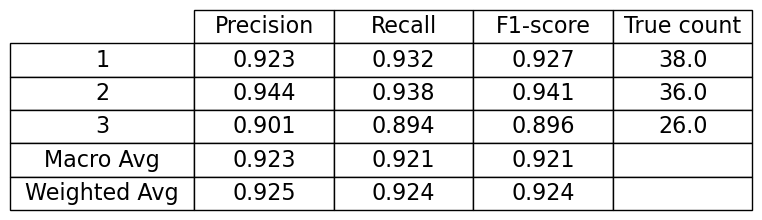
\includegraphics[width=0.9\textwidth]{./figures/q4f_classification_report_reduced_feats}
        \caption{Mean classification report.}
        \label{fig:q4f_classification_report_reduced_feats}
    \end{subfigure}
    \caption{The results shown in Fig. \eqref{fig:q4f_all_feats} but with only the top 382 features.
        The mean test set classification error was 7.6\%.}
    \label{fig:q4f_reduced_feats}
    \end{figure}

    \begin{figure}[htb]
    \centering
    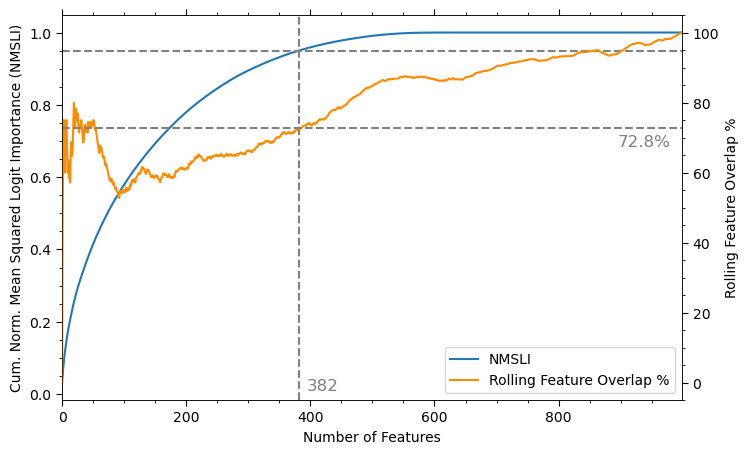
\includegraphics[width=0.9\textwidth]{./figures/q4f_logit_importance}
    \caption{The ordered (highest first), cumulative NMSLI of the features in the \inlinecode{LogisticRegression} model.
        The horizontal grey line is the 95\% threshold, which contains the top 382 features. Amongst the 382 top features
        indicated by the NMSLI, 72.8\% of them were also in the top 382 features for the \inlinecode{RandomForestClassifier}
        indicated by the Gini importance, this is what the rolling feature overlap indicates.}
        \label{fig:q4f_logit_importance}
    \end{figure}

    Everything in the previous section, Sec.\eqref{subsubsec:q4bcde}, was then repeated for a multinomial logistic
    regression classifier: \inlinecode{LogisticRegression}.
    Fig.\eqref{fig:q4f_all_feats} shows the results of the classification using all features, and
    Fig.\eqref{fig:q4f_reduced_feats} shows the results of the classification using only the top 382 features, which
    shows a significant increase in performance in terms of test set classification error and average precision, recall
    and F1-scores.
    The feature importance was computed using a novel metric, the normalised mean squared logit importance (NMSLI).
    This was computed by averaging the squared coefficients across all 3 classes for each feature (by accessing
    \inlinecode{LogisticRegression.coef_}) and then normalising them.
    This provided a feature-wise metric for importance, akin to the Gini importance, which took into account the
    magnitude and consistency of the coefficients across all classes.
    This was then treated the same as the Gini importance, giving the top 382 features which contributed to 95\% of the
    cumulative NMSLI, as shown in Fig.\eqref{fig:q4f_logit_importance}.
    Comparing Fig.\eqref{fig:q4e} and Fig.\eqref{fig:q4f_reduced_feats}, both models performed very similarly across
    all metrics.
